\documentclass{../c-lecture}

\usepackage{algorithm2e}

\subtitle{Introduction}

\begin{document}

\begin{frame}
  \titlepage{}
\end{frame}
\begin{frame}
  \frametitle{Outline}
  \tableofcontents{}
\end{frame}

\section{Introduction}

\begin{frame}
  \frametitle{Who I am?}
  \centering
  \textbf{Parham Alvani}\\
  \textbf{Ph.D. Student in Computer Networks}\\
  \vfill
  \textit{parham [dot] alvani [at] gmail [dot] com}
\end{frame}
\begin{frame}
  \frametitle{Contact Me}
  \begin{itemize}
    \item No instant messaging
    \item \color{Orange} Email is Awesome
  \end{itemize}
\end{frame}

\section{What is this course?}

\begin{frame}
  \frametitle{This Course}
  \begin{itemize}
    \item Introduction to Computer \& Programming
    \item How to use computers to solve our problems
    \begin{itemize}
      \item The problems are computational problems
    \end{itemize}
  \end{itemize}
\end{frame}

\begin{frame}
  \frametitle{This Course (cont’d)}
  \begin{itemize}
    \item What we learn
    \begin{itemize}
      \item Overall overview of computer organization
      \item Problem solving steps
      \begin{itemize}
        \item Algorithm design
          \item A programming language: the {\color{Orange} C}
      \end{itemize}
    \end{itemize}
  \end{itemize}
\end{frame}

\begin{frame}
  \frametitle{This Course (cont’d)}
  \begin{itemize}
    \item What we don’t learn
    \begin{itemize}
      \item In depth computer hardware/software details
      \begin{itemize}
        \color{Aquamarine}
        \item Computer Architecture
        \item Operating System
      \end{itemize}
      \pause%
      \item Most advanced algorithms
      \begin{itemize}
        \color{Aquamarine}
        \item Data Structure
        \item Algorithms
      \end{itemize}
      \pause%
      \item System programming using C
      \begin{itemize}
        \color{Aquamarine}
        \item Operating System
      \end{itemize}
      \pause%
      \item Other programming languages: Java, PHP, etc.
      \begin{itemize}
        \color{Aquamarine}
        \item Advanced Programming
        \item Web Programming
      \end{itemize}
    \end{itemize}
  \end{itemize}
\end{frame}

\begin{frame}
  \frametitle{This Course (cont'd)}
  Steps to learn a new language (English, French, \ldots C, Java, Python, \ldots)

  \begin{enumerate}
    \item Present: what is the new language (course slide)
    \item Practice: how to use the new language in practice (the example)
    \item Produce: use the language to create a new things (Lab, HW)
  \end{enumerate}
\end{frame}

\begin{frame}
  \frametitle{This Course (cont'd)}
  Learning Programming Language

  \begin{itemize}
    \item is not a pure theoretical course (mathematics, \ldots)
    \begin{itemize}
      \item Reading, reading, reading, \ldots
    \end{itemize}
    \item is a practical course needs the product step
    \begin{itemize}
      \item Class, Reading, programming, programming, programming, \ldots
    \end{itemize}
  \end{itemize}
\end{frame}

\begin{frame}
  \frametitle{This Course (cont'd)}
  Course Materials
  \begin{itemize}
    \item Lecture notes (slides) are in (simple) English
  \end{itemize}
\end{frame}
\begin{frame}[allowframebreaks]
  \frametitle{Agenda}
  \begin{itemize}
    \item Introduction
    \item Algorithm Design
    \item Basic Concepts
    \item Calculations
    \item Interaction
    \item Decision
    \item Iteration
    \item Function
    \item Array
    \item Pointer
    \item Struct
    \item File
    \item Misc.
  \end{itemize}
\end{frame}
\begin{frame}
  \frametitle{Grading}
  Major Parts + 5\% Extra
  \begin{table}
    \begin{tabular}{cc}
      \toprule

      Midterm &
      25\% \\

      \midrule

      Final &
      25\% \\

      \midrule

      Lab &
      15\% \\

      \midrule

      Homework &
      30\% \\

      \midrule

      Project &
      10\% \\

      \bottomrule
    \end{tabular}
  \end{table}
\end{frame}

\begin{frame}
  \frametitle{Extra Classes}
  Lab + TA Classes

  \begin{itemize}
    \item Lab:\@ A practical class
    \item TA:\@ More details, Practical aspects, Solving HW
    \item Homework are not accepted after solutions
  \end{itemize}
\end{frame}

\section{Computer organization}

\begin{frame}
  \frametitle{Computers: The Computing Machines}
  Computer Classififcation:
  \begin{itemize}
    \item \textbf{Supercomputers}:\@
    Weather forecast, Large scale simulation, \ldots
    \item \textbf{Mainframe computers}:\@
    The servers in large companies: Google, \ldots
    \item \textbf{Midsize computers}:\@
    The servers in CE department
    \item \textbf{Micro computers (also called PC)}:\@
    Our laptop
    \item \textbf{Pocket PCs}:\@
    Our mobile phones
  \end{itemize}
\end{frame}

\begin{frame}
  \frametitle{Computers}
  \begin{itemize}
    \item Computers are programmable machines capable of performing calculations (computation)
    \item Changing program leads to different operation
    \item Special-purpose machines
    \begin{itemize}
      \item Calculators, game-playing machines, \ldots
    \end{itemize}
    \item General-purpose computers
    \begin{itemize}
      \item Personal computers, notebooks, \ldots
    \end{itemize}
  \end{itemize}
\end{frame}

\begin{frame}
  \frametitle{Data Units}
  \begin{itemize}
    \item Computers are digital machines
    \item Data processed or stored in computer is represented as two-state values
    \begin{itemize}
      \item either 1 or 0 --- BInary digiTs (BIT)
      \item 1 Byte = 8 bits
      \item 1 kilobyte (KB) = 1024 bytes
      \item 1 megabyte (MB) = 1024 kilobyte
      \item 1 gigabyte (GB) = 1024 megabyte
    \end{itemize}
  \end{itemize}
\end{frame}

\begin{frame}
  \frametitle{Data Representation/Coding}
  \begin{itemize}
    \item How to represent our data by 0--1?
    \item In other word, there are some 0 and 1 in the computer, what is the meaning?
    \item {\color{YellowOrange} Coding (Representation Standards)}
    \item Major (common) representations (coding)
    \begin{itemize}
      \item Integer numbers: 1, 1000, -123, 0, \ldots
      \item Floating point numbers: 1.1, 11.232, -12.23, \ldots
      \item Characters: ``A'', ``B'', ``@'', \ldots
    \end{itemize}
  \end{itemize}
\end{frame}

\begin{frame}
  \frametitle{Integer Number Coding}
  \begin{itemize}
    \item There are different representations
    \item One of the (simple) coding is sign-magnitude coding
    \begin{itemize}
      \item If we have $n$ bit for coding integer
      \item The left bit (the MSB): sign
      \item $n-1$ bits: magnitude
    \end{itemize}
  \end{itemize}
  \begin{table}
    \begin{tabular}{ccc}
      \toprule
      4 & 0000 & 0100 \\
      \midrule
      -4 & 1000 & 0100 \\
      \midrule
      0 & 0000 & 0000 \\
      \midrule
      -0 & 1000 & 0000 \\
      \bottomrule
    \end{tabular}
  \end{table}
\end{frame}

\begin{frame}
  \frametitle{Integer Number Coding}
  Two's Complement
\end{frame}

\begin{frame}
  \frametitle{Floating Point Number Coding (IEEE 754)}
  \begin{itemize}
    \item Usually, this coding pattern
    \item Two precisions:
    \begin{figure}
      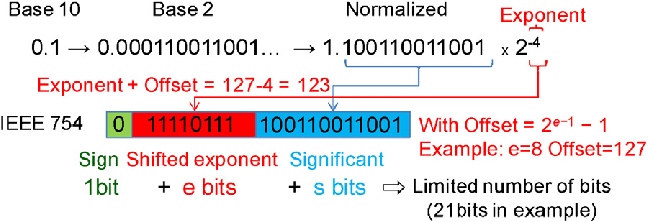
\includegraphics[width=0.75\textwidth]{./img/ieee-754.png}
    \end{figure}
    \begin{itemize}
      \item Single precision: exponent: 8 bit, fraction: 23 bit
      \item Double precision: exponent: 11 bit, fraction: 52 bit
    \end{itemize}
  \end{itemize}
\end{frame}

\begin{frame}
  \frametitle{Character Coding}
    \begin{itemize}
    \item Common character encoding: {\color{Green} ASCII}
    \item 8 bits can represent 256 characters; but,
    \begin{itemize}
      \item There are so many characters (Farsi, Arabic, \ldots)
      \item Solution: UTF (Variable length coding)
      \item 0xxxxxxx: 1 byte code
      \item 110xxxxx 10xxxxxx: 2 byte code
      \item \ldots
    \end{itemize}
  \end{itemize}
\end{frame}

\begin{frame}
  \frametitle{Computer Organization}

  \begin{itemize}
    \item Major Components
    \begin{itemize}
      \item \textbf{Hardware}:
      Physical devices that are wired and performs basic operations
      \item \textbf{Software}:
      Set of programs that run on the hardware
    \end{itemize}
    \item Hardware
    \begin{itemize}
      \item CPU (Central Processing Unit)
      \item Main Memory
      \item Secondary Storage
      \item Input/output
    \end{itemize}
  \end{itemize}
\end{frame}

\begin{frame}
  \frametitle{Computer Organization}
  \begin{figure}
    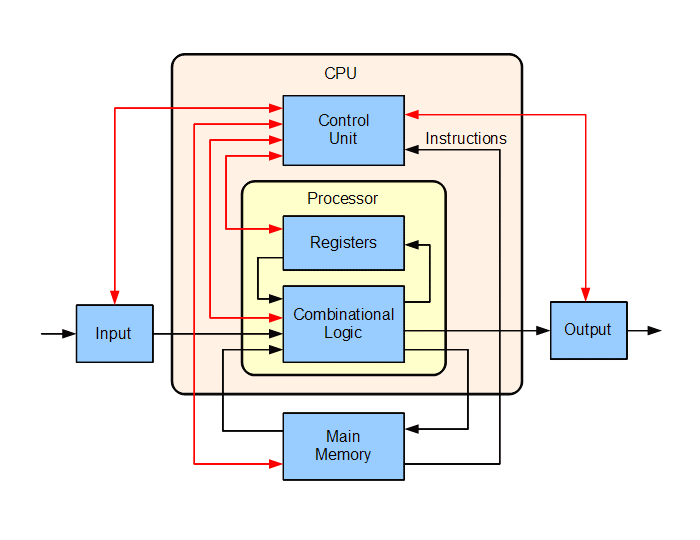
\includegraphics[width=0.75\textwidth]{./img/basic.png}
  \end{figure}
\end{frame}

\begin{frame}
  \frametitle{Computer Organization: CPU}
  \begin{itemize}
    \item ALU (Arithmetic Logic Unit)
    \begin{itemize}
      \item Performs mathematic calculations
      \item Makes decision based on conditions
    \end{itemize}
    \item Special Floating Point processors
    \item Set of working area: Registers
    \item Control Unit
    \begin{itemize}
      \item Controls system operation
    \end{itemize}
    \item Operation and operands are required
    \begin{itemize}
      \item Which are provided by instructions in the main memory
    \end{itemize}
  \end{itemize}
\end{frame}

\begin{frame}
  \frametitle{Computer Organization: Main Memory}
  \begin{itemize}
    \item Ordered sequence of cells (memory cells)
    \item Directly connected to CPU
    \item All programs must be in main memory before execution
    \item When power is turned off, Main memory is cleared
  \end{itemize}
\end{frame}

\begin{frame}
  \frametitle{Computer Organization: Secondary Storage}
  \begin{itemize}
    \item Provides permanent storage for information
    \item Examples of secondary storages:
    \begin{itemize}
      \item Hard Disks
      \item Floppy Disks
      \item Flash/Cool/USB Disks
      \item CD/DVD
      \item Tapes
    \end{itemize}
  \end{itemize}
\end{frame}

\begin{frame}
  \frametitle{Computer Organization: Input Devices}
  \begin{itemize}
    \item Devices that feed data and programs into computers
    \item Examples:
    \begin{itemize}
      \item Keyboard
      \item Mouse
      \item Network Interface Card
      \item Joystick
      \item Microphone
    \end{itemize}
  \end{itemize}
\end{frame}

\begin{frame}
  \frametitle{Computer Organization: Output Devices}
  \begin{itemize}
    \item Devices that computer uses to generate results/outputs
    \item Examples:
    \begin{itemize}
      \item Printer
      \item Monitor
      \item Speaker
      \item Network Interface Card
    \end{itemize}
  \end{itemize}
\end{frame}

\begin{frame}
  \frametitle{Computer Organization: Software}
  \begin{itemize}
    \item What can do the Hardware?
    \begin{itemize}
      \item No useful operation, if there isn’t any software
      \item We should tell/plan/program it to do something
    \end{itemize}
    \item Software
    \begin{itemize}
      \item Programs which are designed for a specific task
    \end{itemize}
    \item Major Software types
    \begin{itemize}
      \item Operating System
      \item Libraries
      \item Applications
    \end{itemize}
  \end{itemize}
\end{frame}

\begin{frame}
  \frametitle{Computer HW \& SW Organization}
  \begin{figure}
    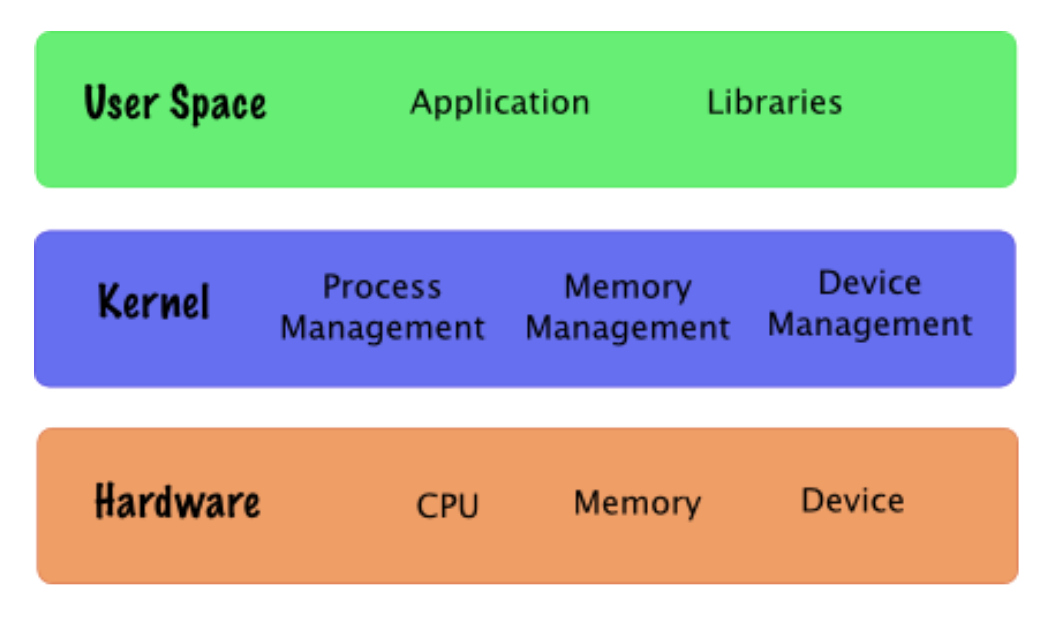
\includegraphics[width=0.75\textwidth]{./img/sw-and-hw.png}
  \end{figure}
\end{frame}

\begin{frame}
  \frametitle{Computer Organization: OS}
  \begin{itemize}
    \item OS
    \begin{itemize}
      \item
        Manages the hardware, HW is a
        {\color{Orange} shared} resource
      \item
        Application programmers can easily use HW, Without knowing the HW
        details
    \end{itemize}
    \item Common operating systems
    \begin{itemize}
      \item Windows XP/Vista/8/10, Linux, Unix, \ldots
    \end{itemize}
  \end{itemize}
\end{frame}

\begin{frame}
  \frametitle{Computer Organization: Libraries}
  \begin{itemize}
    \item The libraries provide the most
      \textit{\color{Green} common} functionalities
    \item In mathematic programs
    \begin{itemize}
      \item \textit{sin}, \textit{cos}, matrix multiplication/inversion
    \end{itemize}
    \item In graphical programs
    \begin{itemize}
      \item Draw a line/cycle, set color, new window
    \end{itemize}
    \item In multimedia programs
    \begin{itemize}
      \item Open/close files, jump, \ldots
    \end{itemize}
  \end{itemize}
\end{frame}

\begin{frame}
  \frametitle{Computer Organization: Applications}
  \begin{itemize}
    \item An application program
    \begin{itemize}
      \item Users use them to do some specific things
      \item \color{Orange} Without knowing the details of the computer
    \end{itemize}
    \item Common application programs
    \begin{itemize}
      \item Word, Internet Explorer, FireFox, Messengers
    \end{itemize}
    \item Common applications in mathematic:
    \begin{itemize}
      \item Matlab, Mathematica, Maple, GAMS, AIMMS
    \end{itemize}
  \end{itemize}
\end{frame}

\begin{frame}
  \frametitle{Programming Execution Phases}
  \begin{enumerate}
    \item Program is loaded from secondary storage to main memory by OS
    \item OS gives the control to the program
    \item Instructions run
    \item
      Required inputs are got from input device \& saved in main memory \&
      used by CPU
    \item Result is saved in main/secondary memory or sent to output devices
  \end{enumerate}
\end{frame}

\begin{frame}
  \frametitle{Programming Execution Phases}
  \begin{figure}
    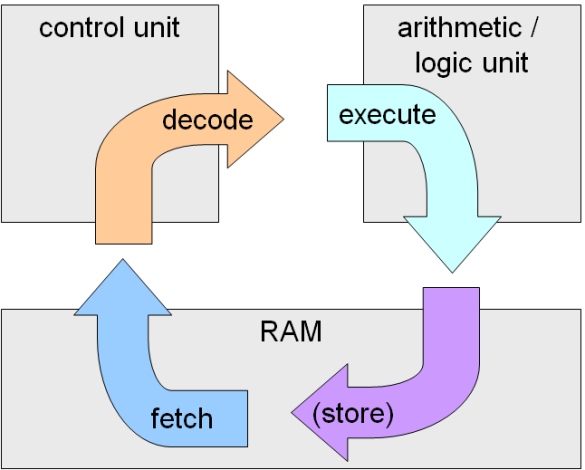
\includegraphics[width=.75\textwidth]{./img/cycle.png}
  \end{figure}
\end{frame}

\begin{frame}
  \frametitle{Programming Execution Phases}
  \begin{itemize}
    \item Basic steps in running instructions:
    \begin{itemize}
      \item
        Read instruction from main memory: \textbf{\color{Green} fetch}
      \item \textbf{\color{Orange} Decode} the instruction
      \item
        Get required \textbf{\color{Blue} operands} from main memory
      \item \textbf{\color{Red} Run} the instruction
      \item Save the \textbf{\color{Cyan} result}
    \end{itemize}
  \end{itemize}
\end{frame}

\begin{frame}
  \frametitle{Von Neumann architecture}
  \begin{itemize}
    \item also known as the von Neumann model or Princeton architecture
    \item
      Keeping both program instructions and data in read-write, random-access
      memory (RAM).
  \end{itemize}
\end{frame}

\begin{frame}
  <h2>How to be general purpose machine?</h2>
  \begin{itemize}
    \item Hardware is simple \& general purpose
    \item Complex tasks (e.g.\ average, sort, \ldots) are programmed by software
    \item Software is translated to the basic instructions
    \item
      This is the way that we
      {\color{Orange} program} computers
  \end{itemize}
\end{frame}

\section{Algorithms \& Programming}

\begin{frame}
  \frametitle{Algorithms}
  \begin{itemize}
    \item Hardware do the basic operations
    \item We want to solve a real problem by computers
    \item We need a solution that
    \begin{itemize}
      \item Specifies how the real (complex) problem should be solved
        {\color{Orange} step-by-step} using the basic operations
    \end{itemize}
    \item The solution is the {\color{Green} ``Algorithm''} of the
      problem
  \end{itemize}
\end{frame}

\begin{frame}
  \frametitle{Algorithms (cont’d)}
  \begin{itemize}
    \item Common Sense (in computer science):
    \begin{enumerate}
      \item The way to do some things
      \item An abstract way to solve a problem
    \end{enumerate}
    \item Formal Definition:
    \begin{quote}
      An algorithm is a \textbf{\color{GreenYellow} finite list} of
      \textbf{\color{GreenYellow} well-defined} instructions for accomplishing
      some task that, given an \textbf{\color{GreenYellow} initial state}, will
      \textbf{\color{GreenYellow} proceed} through a welldefined series of
      successive states, possibly eventually
      \textbf{\color{GreenYellow} terminating} in an end-state
    \end{quote}
  \end{itemize}
\end{frame}

\begin{frame}
  \frametitle{Algorithms: Examples}
  \begin{itemize}
    \item Finding Common Divisor
    \item Finding 2 largest element in a set
    \item Finding shortest path in a graph
    \item Searching in a sorted array
    \item Sorting a set
    \item Combining 2 sorted set in a sorted set
    \item Solving an equation
    \item Compression algorithms
    \item Cryptography algorithms
    \item \ldots
  \end{itemize}
\end{frame}

\begin{frame}
  \frametitle{Algorithms: Description}
  \begin{itemize}
    \item Algorithms are the problem solving steps in our mind!!!
    \item How can we document it (don’t forget it)?
    \item How can we explain/teach it to others peoples?
    \item How can we explain it to computers?
    \item We need some methods to describe algorithms!
    \begin{itemize}
      \item Flow chart
      \item Pseudo-codes
      \item Codes/Programs
    \end{itemize}
  \end{itemize}
\end{frame}

\begin{frame}
  \frametitle{Algorithms: Description (cont’d)}
  \begin{itemize}
    \item Flowcharts:
    \begin{figure}
      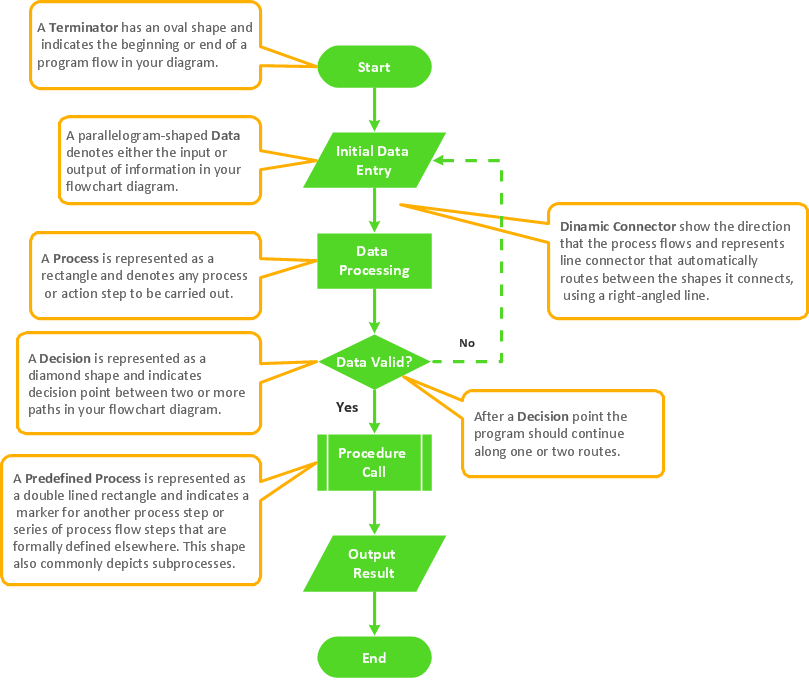
\includegraphics[width=.5\textwidth]{./img/flowchart.png}
    \end{figure}
  \end{itemize}
\end{frame}

\begin{frame}
  \frametitle{Algorithms: Description (cont’d)}
  \begin{itemize}
    \item Pseudo-codes:
    \item A sequence of English and mathematical statements
  \end{itemize}
  \begin{algorithm}[H]
  \KwData{$n \geq 0$}
  \KwResult{$\sum_{i=1}^{n}=i^{2}$}
  $sum \gets 0$\;
  $i \gets 1$\;
  \While{$i \leq n$}{%
    $sq \gets i * i$\;
    $sum \gets sum + sq$\;
    $i \gets i + 1$\;
  }
  \end{algorithm}
\end{frame}

\begin{frame}
  \frametitle{Algorithms: Description (cont’d)}
  \begin{itemize}
    \item Flowcharts and Pseudo-code are for humans not for computer
    \begin{itemize}
      \item Computer \textit{\color{Orange} cannot} run them
    \end{itemize}
    \item What can computer run?
    \begin{itemize}
      \item Instructions in main memory
      \item
        The instructions are in
        \textit{\color{Cyan} ``011100001\ldots''} format
      \item
        To use computers \textmd{We should describe your algorithm in “01” format}
    \end{itemize}
  \end{itemize}
\end{frame}

\begin{frame}
  \frametitle{Algorithms: Description (cont’d)}
  \begin{figure}
    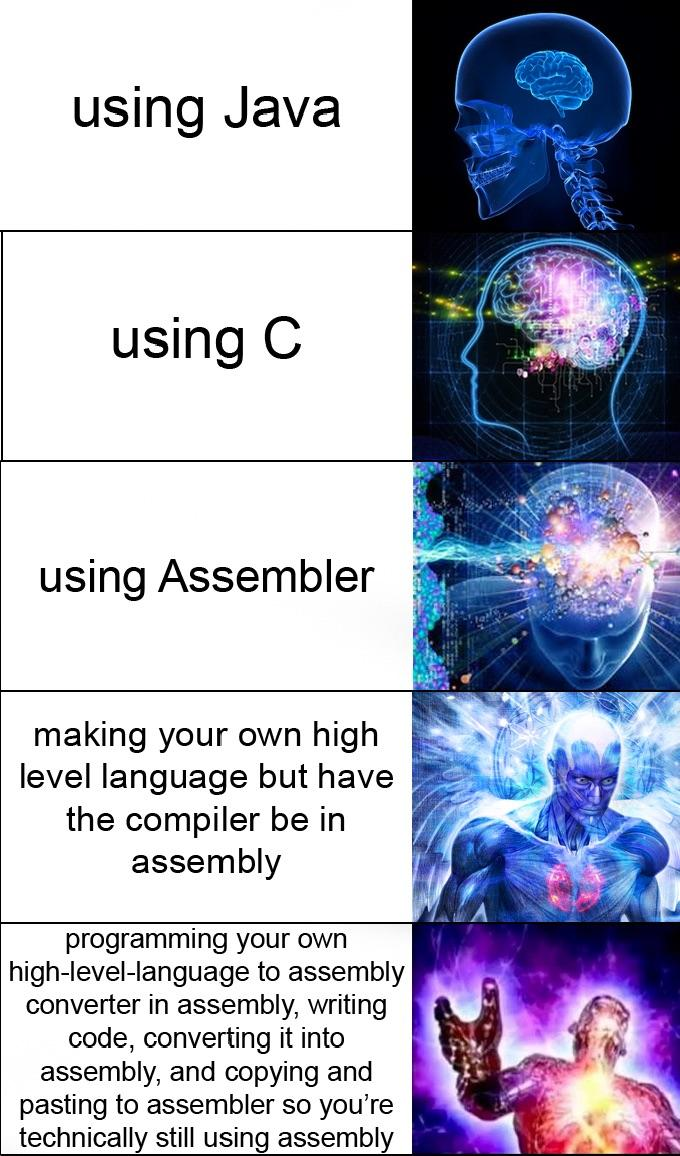
\includegraphics[width=.35\textwidth]{./img/assembly.jpg}
  \end{figure}
\end{frame}

\begin{frame}
  \frametitle{Programming Language}
  \begin{itemize}
    \item
      Programming languages are the tools to describe your algorithms for
      computers
    \begin{itemize}
      \item Software is developed by programming languages
    \end{itemize}
    \item New languages which is understandable by computers
    \item Human languages are not used. Why?
    \item When algorithm is described with a programming language
    \begin{itemize}
      \item
        It cannot be run on computer directly if the languages is not 011001001
      \item
        There are some other programs that translate the programming language to
        ``010\ldots''
      \item The output ``0101\ldots'' can run on computers
    \end{itemize}
  \end{itemize}
\end{frame}

\begin{frame}
  \frametitle{Programming Language: Machine Level}
  \begin{itemize}
    \item Computer’s native language
    \item What is saved in the main memory
    \item
      The processor architecture specifies the format of 01s, machine depended
    \item Example
    \begin{itemize}
      \item Add two numbers: 00100111 1010 0101
    \end{itemize}
    \item Completely incomprehensible to (most) people
  \end{itemize}
\end{frame}

\begin{frame}
  \frametitle{Programming Language: Assembly}
  \begin{itemize}
    \item Programming based on mnemonics
    \item
      There are {\color{Orange} one-to-one mapping} between
      machine language and assembly mnemonics
  \end{itemize}
\end{frame}

\begin{frame}
  \frametitle{Programming Language: High Level}
  \begin{itemize}
    \item Easy for programming, English-like keywords
    \item
      There isn’t one-to-one relation between high level statements and machine
      level statements
    \item Example: C, C++, Pascal, Java, PHP, Python, Go, \ldots
  \end{itemize}
\end{frame}

\begin{frame}
  \frametitle{Translation of High Level Languages}
  \begin{itemize}
    \item Two types of translators
    \begin{itemize}
      \item Interpreter
      \item Compiler
    \end{itemize}
    \item Interpreter
    \begin{itemize}
      \item Checks and runs program lines one-by-one
      \item Easy, slow, and we need the interpreter
    \end{itemize}
    \item Compiler
    \begin{itemize}
      \item Check all lines, creates executable output file
      \item Fast and Stand alone program
    \end{itemize}
  \end{itemize}
\end{frame}

\begin{frame}
  \frametitle{Compiler}
  \begin{itemize}
    \item
      A {\color{Orange} set} of computer programs do the
      {\color{Green} Compilation}
    \item
      \textbf{\color{Orange} Preprocessor}: Prepare file for compiler
    \item \textbf{\color{Orange} Compiler}: Create assembly code
    \item
      \textbf{\color{Green} Assembler}: Convert assembly code to binary
      code
    \item
      \textbf{\color{Green} Linker}: Collect all required binary files
      (from libraries) into a single loadable file
    \item Each language has its own compiler
  \end{itemize}

  \begin{block}{}
  Usually compiler do all above steps, you just compile the file and get a
  executable file
  \end{block}
\end{frame}

\begin{frame}
  \frametitle{Compiler}
  \begin{figure}
    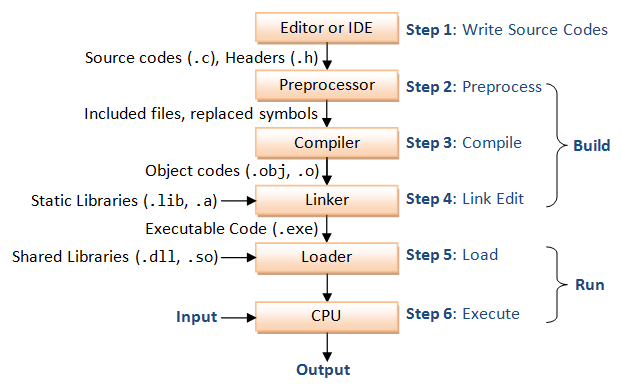
\includegraphics[width=.75\textwidth]{./img/build-flow.png}
  \end{figure}
\end{frame}

\section{Solving problems}

\begin{frame}
  \frametitle{Solving Problems}
  \begin{itemize}
    \item How to solve problems using computers
    \begin{itemize}
      \item Develop a {\color{Orange} program} for it
    \end{itemize}
    \item Steps
    \begin{enumerate}
      \item Analysis: Input, output
      \item Algorithm Design
      \item Coding
      \item Compile (Program)
      \item Execution (Test)
      \item Documentation
    \end{enumerate}
  \end{itemize}
\end{frame}

\begin{frame}
  \frametitle{Solving Problems: Analysis}

  \begin{itemize}
    \item Problem solving process consists of: Input, Algorithm, Output
    \item Determine what information is available as the input to your algorithm
    \item Determine what information is desired as the output from your algorithm
    \item
      What needs to be done on the input to produce the output?
      \textbf{\color{Orange} Algorithm}
  \end{itemize}
\end{frame}

\begin{frame}
  \frametitle{Solving Problems: Algorithm}
  \begin{itemize}
    \item
      Determine a series of steps that transforms the input data into the output
      results
    \item
      Find all the \textit{\color{RubineRed} special cases} that the must be
      handled
    \item
      If necessary modify or redesign your series of steps so that all special
      cases are handled
    \item Verify your algorithm
  \end{itemize}
\end{frame}

\begin{frame}
  \frametitle{Solving Problems: Coding}
  \begin{itemize}
    \item Describe your algorithm by a programming language
    \item
      You must code exactly in the programming language
      \textit{\color{Orange} syntax}
    \item Compiler itself is a program it isn’t a human
    \begin{itemize}
      \item It is not intelligent
      \item It just does the steps of the compiling algorithm
      \item It does not understand what do you mean!!!
    \end{itemize}
  \end{itemize}
\end{frame}

\begin{frame}
  \frametitle{Solving Program: Execution}
  \begin{itemize}
    \item Compiler generated the executable file
    \item Run the executable code
    \begin{itemize}
      \item First try to use simple
      \item Then try larger and complex inputs
    \end{itemize}
  \end{itemize}
\end{frame}

\begin{frame}
  \frametitle{Solving Program}
  \begin{figure}
  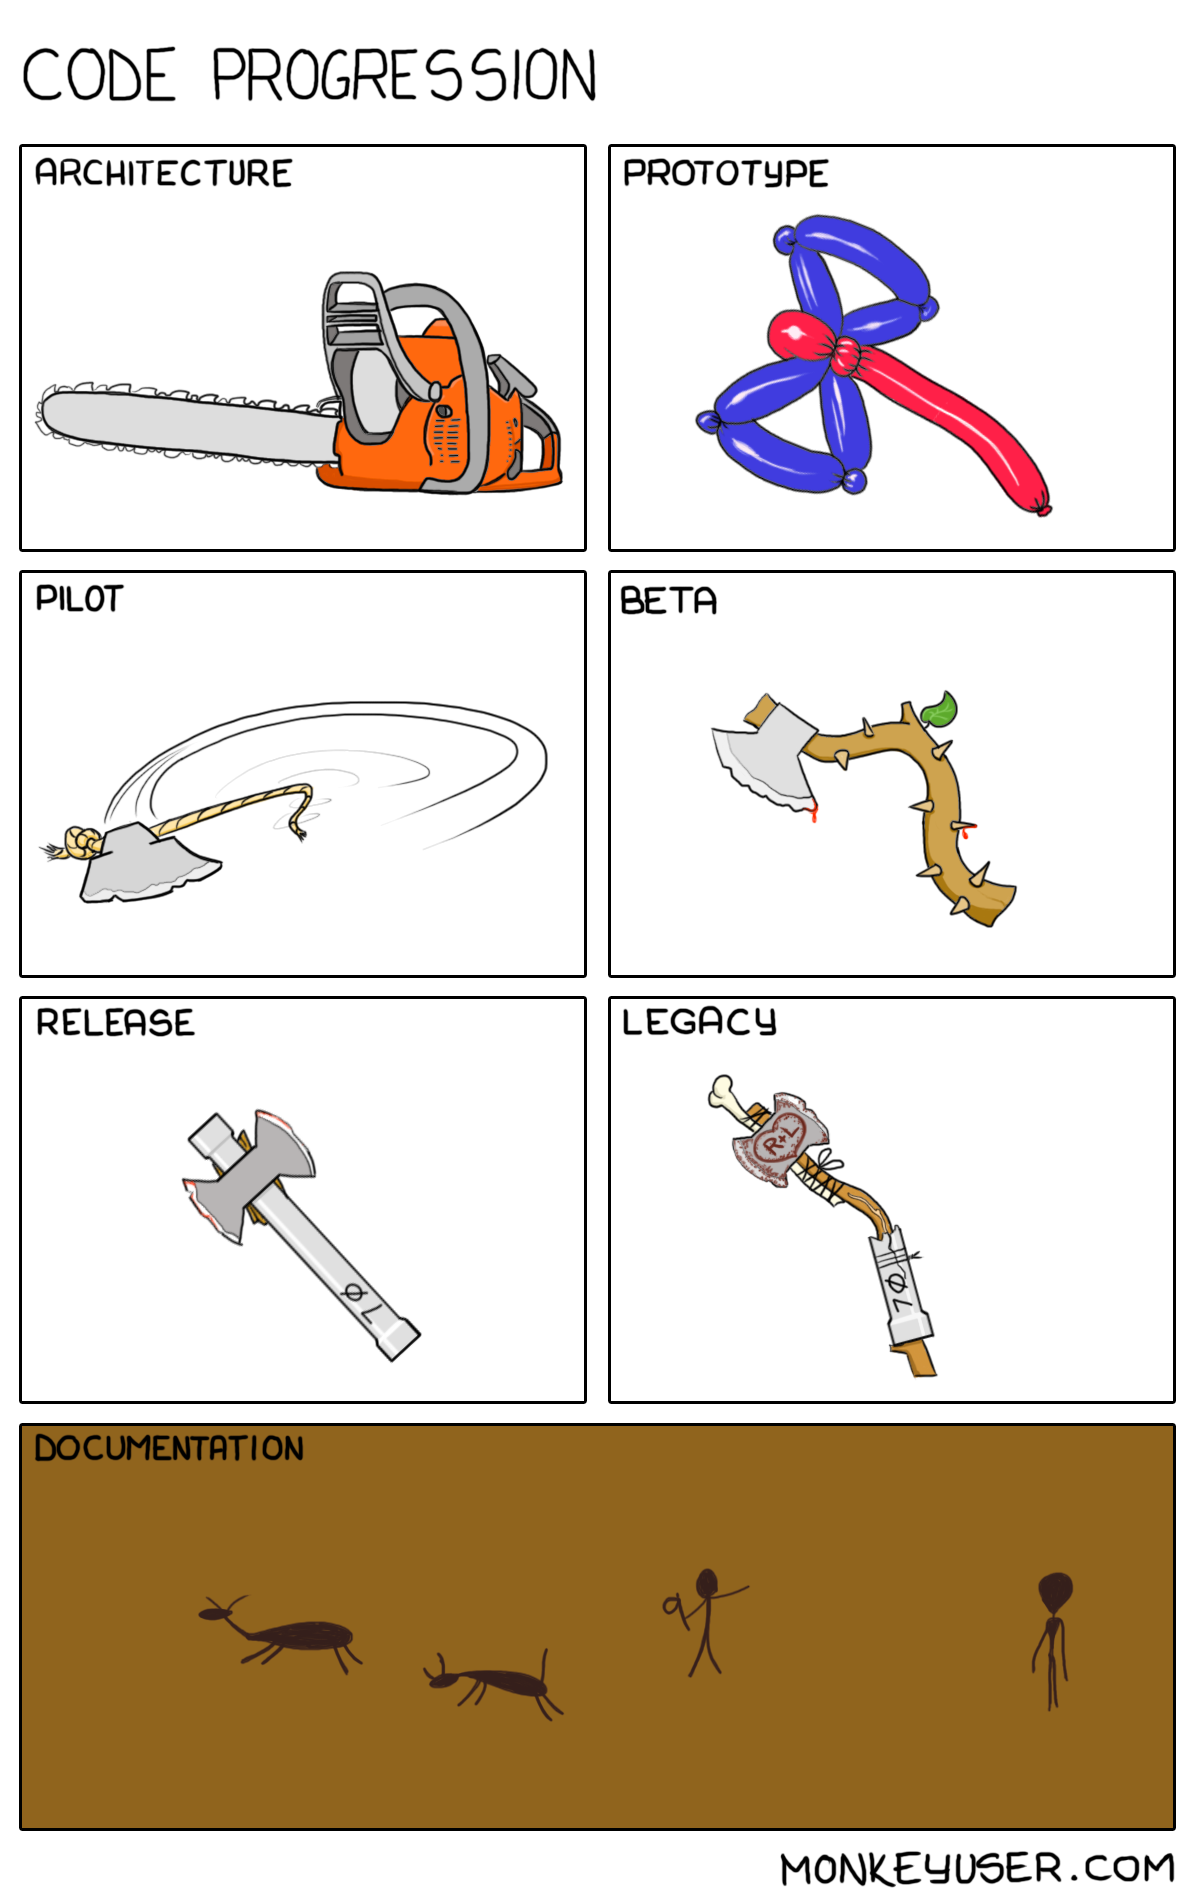
\includegraphics[height=.75\textheight]{./img/code-progress.png}
  \end{figure}
\end{frame}

\begin{frame}
  \frametitle{Errors in Solving Problems}
  \begin{itemize}
    \item Compile / Syntax error: Compiler does not recognize your code
    \item Link error: Linker cannot find the required libraries
    \item Runtime error: Program does not run correctly
    \begin{itemize}
      \item Example: Division by zero
    \end{itemize}
    \item Logical Error: Program does not produce the expected result
    \begin{itemize}
      \item It is called \textit{\color{Red} bug}
      \item No one (compiler, assembler) except debugger can help you
    \end{itemize}
  \end{itemize}
\end{frame}

\begin{frame}
  \frametitle{Errors in Solving Problems}
  \begin{itemize}
    \item Why error?
    \begin{itemize}
      \item You do not understand and analysis the problem correctly
      \item You do not develop a right algorithm for the problem
      \item You have mistakes in your coding
    \end{itemize}
  \end{itemize}
\end{frame}

\begin{frame}
  \frametitle{Debugging}
  \begin{itemize}
    \item The process of resolving the errors
    \begin{itemize}
      \item Example: A program to divide two numbers</dd>
    \end{itemize}

    \item Compile/Syntax error
    \begin{itemize}
      \item Compiler tells where it is, check syntax
    \end{itemize}

    \item Link error
    \begin{itemize}
      \item Compiler tells what it is, check syntax \& libraries
    \end{itemize}

    \item Run time error
    \begin{itemize}
      \item
        Try to find it, use debugger to run step-by-step, print debug messages
      \item Check syntax \& semantic of the line
    \end{itemize}
  \end{itemize}
\end{frame}

\begin{frame}
  \frametitle{Debugging}
  \begin{itemize}
    \item Logical error
      \begin{itemize}
        \item
          Try to find it, use debugger to run step-by-step, print debug messages
        \item Check syntax \& semantic of program
        \item Revise the algorithm
      \end{itemize}
  \end{itemize}
\end{frame}

\begin{frame}
  \frametitle{Desired Features of Programs}
  \begin{itemize}
    \item \textbf{Integrity}
    Correctly solve the problem
    \item \textbf{Clarity}
    Easy to read
    \item \textbf{Simplicity}
    Easy to understand
    \item \textbf{Efficiency}
    Speed and memory
    \item \textbf{Modularity}
    Break down of a large task
    \item \textbf{Generality}
    Tunable by input as much as possible
  \end{itemize}
\end{frame}

\begin{frame}
  \frametitle{Summary}
  \begin{itemize}
    \item Computer organization
    \begin{itemize}
      \item Hardware and Software
    \end{itemize}
    \pause%
    \item Algorithm \& Program
    \begin{itemize}
      \item What is the difference between them
    \end{itemize}
    \pause%
    \item How to solve a problem using computer
    \begin{itemize}
      \item Steps
    \end{itemize}
    \pause%
    \item Errors in problem solving
    \item What is the next: Design algorithm
  \end{itemize}
\end{frame}

\begin{frame}
  \frametitle{Legends}
  \begin{figure}
    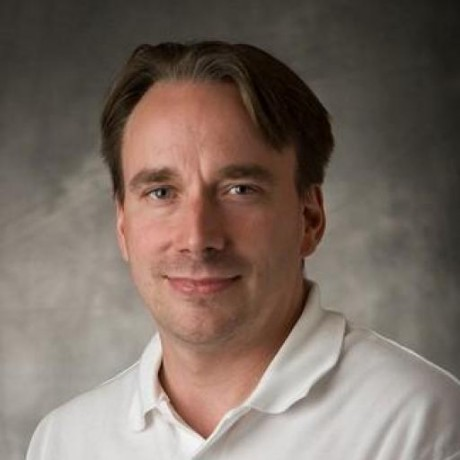
\includegraphics[height=.75\textheight]{./img/torvalds.png}
  \end{figure}
  \pause%
  \centering
  \color{Violet} Linus Torvalds
\end{frame}

\end{document}
